\documentclass[9pt,twocolumn,twoside,lineno]{pnas-new}
% Use the lineno option to display guide line numbers if required.

\templatetype{pnasresearcharticle} % Choose template 
% {pnasresearcharticle} = Template for a two-column research article
% {pnasmathematics} %= Template for a one-column mathematics article
% {pnasinvited} %= Template for a PNAS invited submission
\graphicspath{{/Users/jm200/Library/CloudStorage/Dropbox/Miller Lab/github/POAR-Forecasting/Manuscript/Figures/}}
\newcommand{\tom}[2]{{\color{red}{#1}}\footnote{\textit{\color{red}{#2}}}}
\newcommand{\jacob}[2]{{\color{blue}{#1}}\footnote{\textit{\color{blue}{#2}}}}
\title{Forecasting range shifts of a dioecious plant species under climate change}

% Use letters for affiliations, numbers to show equal authorship (if applicable) and to indicate the corresponding author
\author[a,c,1]{Jacob K. Moutouama\, \textit{0000-0003-1599-1671}}
\author[b]{Aldo Compagnoni\,\textit{0000-0001-8302-7492}} 
\author[a]{Tom E.X. Miller\,\textit{0000-0003-3208-6067}}

\affil[a]{Program in Ecology and Evolutionary Biology, Department of BioSciences, Rice University, Houston, Texas, USA}
\affil[b]{Institute of Biology, Martin Luther University Halle-Wittenberg, Halle, Germany; and German Centre for Integrative Biodiversity Research (iDiv), Leipzig, Germany}

% Please give the surname of the lead author for the running footer
\leadauthor{Moutouama} 

% Please add here a significance statement to explain the relevance of your work
\significancestatement{The vast majority of models used to forecast population viability and range shifts in response to climate change overlook the complexity of sex structure, and thus the potential for females and males to differ in their sensitivity to climate drivers. Here, we combined a common garden experiment with mathematical models to demonstrate that accounting for only one sex could lead to an underestimation of the impact of climate change on dioecious species, particularly in regions of their range that are biased toward one sex. }

% Please include corresponding author, author contribution and author declaration information
\authorcontributions{J.K.M., A.C. and T.E.X.M. designed the study.\\
A.C. and T.E.X.M. collected the data. \\
All authors conducted the statistical analyses and modeling.\\
J.K.M. drafted the manuscript, and T.E.X.M contributed to revisions.}
\authordeclaration{The authors declare no conflict of interest }
%\equalauthors{\textsuperscript{1}A.O.(Author One) and A.T. (Author Two) contributed equally to this work (remove if not applicable).}
\correspondingauthor{\textsuperscript{2}To whom correspondence should be addressed. E-mail: jmoutouama@gmail.com}

% Keywords are not mandatory, but authors are strongly encouraged to provide them. If provided, please include two to five keywords, separated by the pipe symbol, e.g:
\keywords{demography $|$  forecasting $|$  global warming $|$ matrix projection model$|$ population dynamics $|$ sex ratio $|$ range limits $|$ } 

\begin{abstract}
%250 words limit . The number now is 192
Global climate change has triggered an urgent need for predicting the reorganization of Earth's biodiversity.
For dioecious species (in which female and male reproductive organs are not on the same individual), it is unclear how commonly unique climate sensitivities of females and males could influence projections for species-level responses to climate change. 
We developed demographic models of range limitation, parameterized from geographically distributed common garden experiments, with females and males of a dioecious grass species (\textit{Poa arachnifera}) throughout and beyond its range in the south-central U.S. 
Female-dominant and two-sex model versions both predict that future climate change will alter population viability and will induce a poleward niche shift beyond current northern limits.
However, the magnitude of niche shift was underestimated by the female-dominant model, because females have broader temperature tolerance than males and become mate-limited under female-biased sex ratios.
Our result illustrate how explicit accounting for both sexes could enhance population viability forecasts and conservation planning for dioecious species in response to climate change.
\end{abstract}

%\dates{This manuscript was compiled on \today}
\doi{\url{www.pnas.org/cgi/doi/10.1073/pnas.XXXXXXXXXX}}

\begin{document}

\maketitle
\thispagestyle{firststyle}
\ifthenelse{\boolean{shortarticle}}{\ifthenelse{\boolean{singlecolumn}}{\abscontentformatted}{\abscontent}}{}

% If your first paragraph (i.e. with the \dropcap) contains a list environment (quote, quotation, theorem, definition, enumerate, itemize...), the line after the list may have some extra indentation. If this is the case, add \parshape=0 to the end of the list environment.
\dropcap{R}ising temperatures and extreme drought events associated with global climate change are leading to increased concern about how species will become redistributed across the globe under future climate conditions \citep{bertrand2011changes,gamelon2017interactions,smith2024extreme}.
Species' range limits, when not driven by dispersal limitation, should generally reflect the limits of the ecological niche \citep{lee2016synthesis}.
Niches and geographic ranges are often limited by climatic factors including temperature and precipitation \citep{sexton2009evolution}. 
Therefore, any substantial changes in the magnitude of these climatic factors could impact population viability, with implications for range expansions or contractions based on which regions of a species' range become more or less suitable  \citep{davis2001range, pease1989model}. 

%Dioecious species (most animals and ca. 7\% of plant species) might be particularly vulnerable to the influence of climate change because they often display skewed sex ratios that are generated or reinforced by sexual niche differentiation, i.e., the distinct responses of females and males to shared climate drivers) \citep{Tognetti2012}. 
Forecasting range shifts for dioecious species (most animals and ca. 7\% of plant species) is complicated by the potential for sexual niche differentiation, i.e. distinct responses of females and males to shared climate drivers \citep{Tognetti2012,pottier2021sexual,hultine2016climate,morrison2016causes}. 
%The lower cost of reproduction for one sex (male or female) may allow that sex to invest its energy in other functions that produce higher growth rates, greater clonality, or even higher survival rates compared to the other sex, leading to sexual niche differentiation \citep{bruijning2017surviving}.
Accounting for sexual niche differentiation is a long-standing challenge in accurately predicting which sex will successfully track environmental change and how this will impact population viability and range shifts \citep{jones1999sex,gissi2023exploring}. 
Populations in which males are rare under current climatic conditions could experience low reproductive success due to sperm or pollen limitation that may lead to population decline in response to climate change that disproportionately favors females \citep{eberhart2017sex}.
In contrast, climate change could expand male habitat suitability (e.g. upslope movement), which might increase seed set for mate-limited females and favor range expansion \citep{petry2016sex}. 
Across dioecious plants, for example, studies suggest that future climate change toward hotter and drier conditions may favor male-biased sex ratios \citep{field2013comparative,hultine2016climate}. 
Although the response of species to climate warming is an urgent and active area of research, few studies have disentangled the interaction between sex and climate drivers to understand their combined effects on population dynamics and range shifts, despite calls for such an approach \citep{hultine2016climate,gissi2023exploring}.

The vast majority of theory and models in population biology, including those used to forecast biodiversity responses to climate change, ignore the complication of sex structure \citep[but see][] {pottier2021sexual,ellis2017does,Elena}.
Traditional approaches instead focus exclusively on females, assuming that males are in sufficient supply as to never limit female fertility. 
In contrast, ``two-sex'' models are required to fully account for demographic differences between females and males and sex-specific responses to shared climate drivers \citep{gerber2014two,miller2011sex}. 
Sex differences in maturation, reproduction, and mortality schedules can generate skew in the operational sex ratio (OSR; sex ratio of individuals available for mating) even if the birth sex ratio is 1:1 \citep{eberhart2017sex,shelton2010ecological}. 
Climate and other environmental drivers can therefore influence the OSR via their influence on sex-specific demographic rates. 
In a two-sex framework, demographic rates both influence and respond to the OSR in a feedback loop that makes two-sex models inherently nonlinear and more data-hungry than corresponding female-dominant models. 
Given the additional complexity and data needs, forecasts of range dynamics for dioecious species under future climate change that explicitly account for females, males, and their inter-dependence are limited \citep{petry2016sex,lynch2014climate}.

Tracking the impact of climate change on  population viability ($\lambda$) and distributional limits of dioecious taxa depends on our ability to build mechanistic models that take into account the spatial and temporal context of sex specific response to climate change, while accounting for sources of uncertainty \citep{davis2001range,evans2016towards}.
Structured population models built from demographic data collected from geographically distributed observations or common garden experiments provide several advantages for studying the impact of climate change on species' range shifts \citep{merow2017climate,schwinning2022common,schultz2022climate}.
First, demographic models link individual-level life history events (mortality, development, and regeneration) to population demography, allowing the investigation of factors explaining vital rate responses to environmental drivers \citep{ehrlen2015predicting,louthan2022climate,dahlgren2016demography}. 
Second, demographic models have a natural interface with %experimental treatments that can isolate spatial and temporal correlations between environmental factors, thus overcoming a main disadvantage with many types of correlative studies \citep{leicht2007comparative}. 
%Third, demographic models are typically constructed from 
statistical estimation of individual-level vital rates that provide quantitative measures of uncertainty and isolate different sources of variation, features that can be propagated to population-level predictions \citep{elderd2016quantifying,ellner2022critical}.
% The uncertainty around lambda can be used to estimate the probability of self-sustaining populations, conditional on different factors of the environment.
Finally, structured demographic models can be used to identify which aspects of climate are the most important drivers of population dynamics.
For example, Life Table Response Experiments (LTRE) built from structured models have become widely used to understand the relative importance of covariates in explaining variation in population growth rate  \citep{ellner2016data,hernandez2023exact,czachura2020demographic}.
%LTRE is also used to get a mechanistic understanding of how a given treatment (eg. temperature or precipitation) could affect population dynamics through unique vital rate responses \citep {caswell1989analysis,o2024nonlinear,morrison2007demographic,iler2019reproductive}. %\jacob{}{Yes I don't want to get distracted by SDMs. The story is still interesting without bashing the SDMs studies. That being said, I showed the advantage of using demographic models over traditional correlative approaches. Line 59-62)}
% At their range edge where climatic conditions are expected to be less favorable, if dioecious species populations are non-viable in response to climate change, global warming will induce range contraction in dioecious species.
% In reverse, if populations at the edge are viable habitats in response to global warming, dioecious species populations could shift their range and relocate to more favorable and thereby favored range expansion. 

In this study, we combined geographically-distributed common garden experiments, hierarchical Bayesian statistical modeling, two-sex population projection modeling, and climate back-casting and forecasting to understand demographic responses to climate change and their implications for past, present, and future range dynamics. 
Our work focused on the dioecious plant Texas bluegrass (\textit{Poa arachnifera}), which is distributed along environmental gradients in the south-central U.S. corresponding to variation in temperature across latitude and precipitation across longitude (Fig. \ref{fig:study_design}A)\jacob{}{Fig. A  does not show what we are saying here. Maybe I should add the Figure with the raster}. 
%This region has experienced rapid climate warming since 1900 and this is projected to continue through the end of the century (Fig. \ref{fig:study_design} B and C). 
Our previous study showed that, despite evidence for differentiation of climatic niche between sexes, the female niche mattered the most in driving longitudinal range limits of Texas bluegrass \citep{miller2022two}. 
However, that study used a single proxy variable (longitude) to represent environmental variation related to aridity and did not consider variation in temperature, which is the %much stronger dimension of forecasted climate change in this region (Fig. \ref{Sup:climate_normal_weather}). 
Developing a rigorous forecast for the implications of future climate change requires that we transition from implicit to explicit treatment of multiple climate drivers, as we do here.
Leveraging the power of Bayesian inference, we take a probabilistic view of past, present, and future range limits by quantifying the probability of population viability ($Pr(\lambda\ge1)$) in relation to climate drivers of demography, an approach that fully accounts for uncertainty arising from multiple sources of estimation and process error. %using Markov Chain Monte Carlo (MCMC) can be utilized to infer species niche which is defined as the range of resources and conditions allowing its populations of self-sustaining populations, conditional on different factors of the environment \citep{maguire1973niche,hutchinson1978introduction,diez2014probabilistic}
Specifically, we asked: 
\begin{enumerate}
	\item What are the sex-specific vital rate responses to variation in temperature and precipitation across the species' range?
	\item How do sex-specific vital rates combine to determine the influence of climate variation on population growth rate ($\lambda$)?
	\item What is the impact of climate change on operational sex ratio throughout the range?
	\item What are the likely historical and projected dynamics of the Texas bluegrass geographic niche and how does accounting for sex structure modify these predictions?
\end{enumerate}


\begin{figure}[H]
  \begin{center}
    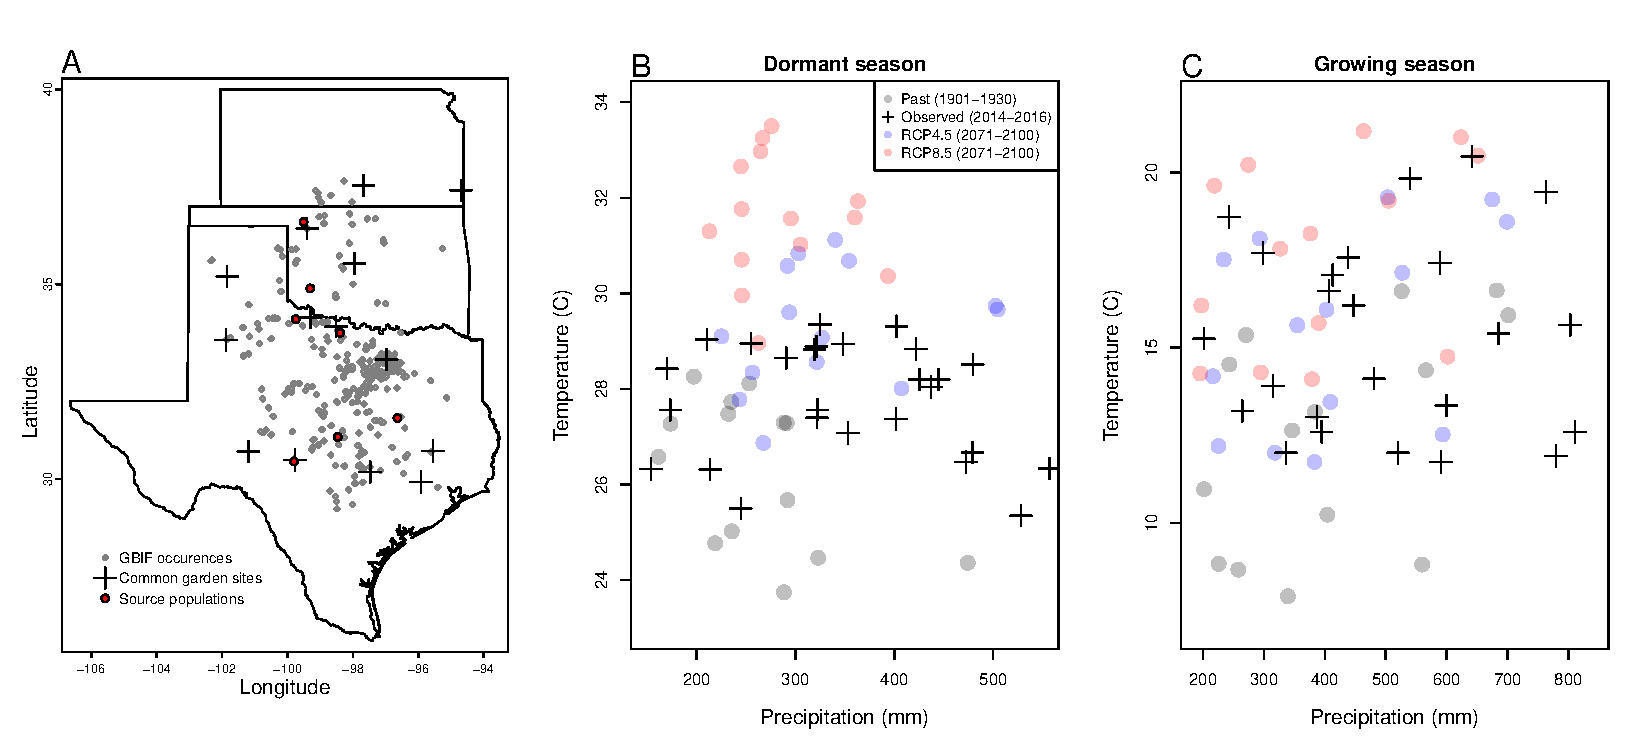
\includegraphics[width=1\linewidth]{tom_map_v2.pdf}
  \caption{Experimental gardens and climate of the study region. 
  	\textbf{A}: Map of 14 experimental garden sites (crosses) in Texas, Oklahoma, and Kansas relative to GBIF occurrences of \textit{Poa arachnifera} (gray points). Red points indicate source populations for plants used in the common garden experiment. 
  	\textbf{B,C}: Past, future, and observed climate space for growing and dormant seasons. Crosses show observed conditions for the sites and years of the common garden experiment. Gray points show historical (1901-1930) climate normals, and blue and red points show end-of-century (2071-2100) climate normals for RCP4.5 and RCP8.5 projections, respectively, form MIROC5. 
 % See also (Figure \ref{Sup:clim_change} for more information about historical and projected climate change in the study region.
 }
  \label{fig:study_design}
  \end{center}
\end{figure}



\showmatmethods{} % Display the Materials and Methods section

\acknow{This research was supported by National Science Foundation Division of Environmental Biology awards 2208857 and 2225027. 
We thank the institutions who hosted us at their field station facilities, including
}

\showacknow{} % Display the acknowledgments section

% Bibliography
\bibliography{pnas}

\end{document}